\documentclass[a4paper,11pt]{scrartcl}%scrbook %[...,twoside]

\usepackage[a4paper,left=3.5cm,right=2.5cm,bottom=3.5cm,top=3cm]{geometry}

\usepackage[ngerman]{babel}

% Caption Packet
\usepackage[margin=0pt,font=small,labelfont=bf]{caption}
% Gliederung einstellen
%\setcounter{secnumdepth}{5}
%\setcounter{tocdepth}{5}
%\usepackage[Sonny]{fncychap}
%\ChTitleVar{\huge\rm}
\usepackage[pdftex]{graphicx,color}
\usepackage{amsmath,amssymb}
% Theorem-Umgebungen
\usepackage[amsmath,thmmarks]{ntheorem}
% Korrekte Darstellung der Umlaute
\usepackage[utf8]{inputenc}
\usepackage[T1]{fontenc}
\usepackage{lmodern}
\usepackage[onehalfspacing]{setspace}
% Algorithmen
\usepackage{algorithm}
\usepackage{algorithmic}
%\renewcommand{\algorithmiccomment}[1]{\hfill \tiny//~#1\normalsize}
% Bibtex deutsch
\usepackage{bibgerm}
% URLs
\usepackage{url}
\usepackage{verbatim}
\usepackage{algorithm}

% Theorem-Optionen %
\theoremseparator{}
\theoremstyle{change}
\newtheorem{theorem}{Theorem}[section]
\newtheorem{satz}[theorem]{Satz}
\newtheorem{lemma}[theorem]{Lemma}
\newtheorem{korollar}[theorem]{Korollar}
\newtheorem{proposition}[theorem]{Proposition}
% Ohne Numerierung
\theoremstyle{nonumberplain}
\renewtheorem{theorem*}{Theorem}
\renewtheorem{satz*}{Satz}
\renewtheorem{lemma*}{Lemma}
\renewtheorem{korollar*}{Korollar}
\renewtheorem{proposition*}{Proposition}
% Definitionen mit \upshape
\theorembodyfont{\upshape}
\theoremstyle{change}
\newtheorem{definition}[theorem]{Definition}
\theoremstyle{nonumberplain}
\renewtheorem{definition*}{Definition}
% Kursive Schrift
\theoremheaderfont{\itshape}
\newtheorem{notation}{Notation}
\newtheorem{konvention}{Konvention}
\newtheorem{bezeichnung}{Bezeichnung}
\theoremsymbol{\ensuremath{\Box}}
\newtheorem{beweis}{Beweis}
\theoremsymbol{}
\theoremstyle{change}
\theoremheaderfont{\bfseries}
\newtheorem{bemerkung}[theorem]{Bemerkung}
\newtheorem{beobachtung}[theorem]{Beobachtung}
\newtheorem{beispiel}[theorem]{Beispiel}
\newtheorem{problem}{Problem}
\theoremstyle{nonumberplain}
\renewtheorem{bemerkung*}{Bemerkung}
\renewtheorem{beispiel*}{Beispiel}
\renewtheorem{problem*}{Problem}
%
%% Algorithmen anpassen %
%\renewcommand{\algorithmicrequire}{\textit{Eingabe:}}
%\renewcommand{\algorithmicensure}{\textit{Ausgabe:}}
%\floatname{algorithm}{Algorithmus}
%\renewcommand{\listalgorithmname}{Algorithmenverzeichnis}
%\renewcommand{\algorithmiccomment}[1]{\color{grau}{// #1}}
%
% Floating-Umgebungen anpassen %
\renewcommand{\topfraction}{0.9}
\renewcommand{\bottomfraction}{0.8}
% Abkuerzungen richtig formatieren %
\usepackage{xspace}
\newcommand{\vgl}{vgl.\@\xspace} 
\newcommand{\zB}{z.\nolinebreak[4]\hspace{0.125em}\nolinebreak[4]B.\@\xspace}
\newcommand{\bzw}{bzw.\@\xspace}
\newcommand{\dahe}{d.\nolinebreak[4]\hspace{0.125em}h.\nolinebreak[4]\@\xspace}
\newcommand{\etc}{etc.\@\xspace}
\newcommand{\evtl}{evtl.\@\xspace}
\newcommand{\ggf}{ggf.\@\xspace}
\newcommand{\bzgl}{bzgl.\@\xspace}
\newcommand{\so}{s.\nolinebreak[4]\hspace{0.125em}\nolinebreak[4]o.\@\xspace}
\newcommand{\iA}{i.\nolinebreak[4]\hspace{0.125em}\nolinebreak[4]A.\@\xspace}
\newcommand{\sa}{s.\nolinebreak[4]\hspace{0.125em}\nolinebreak[4]a.\@\xspace}
\newcommand{\su}{s.\nolinebreak[4]\hspace{0.125em}\nolinebreak[4]u.\@\xspace}
\newcommand{\ua}{u.\nolinebreak[4]\hspace{0.125em}\nolinebreak[4]a.\@\xspace}
\newcommand{\og}{o.\nolinebreak[4]\hspace{0.125em}\nolinebreak[4]g.\@\xspace}
\newcommand{\oBdA}{o.\nolinebreak[4]\hspace{0.125em}\nolinebreak[4]B.\nolinebreak[4]\hspace{0.125em}d.\nolinebreak[4]\hspace{0.125em}A.\@\xspace}
\newcommand{\OBdA}{O.\nolinebreak[4]\hspace{0.125em}\nolinebreak[4]B.\nolinebreak[4]\hspace{0.125em}d.\nolinebreak[4]\hspace{0.125em}A.\@\xspace}

% Leere Seite ohne Seitennummer, naechste Seite rechts
\newcommand{\blankpage}{
 \clearpage{\pagestyle{empty}\cleardoublepage}
}
\bibliographystyle{unsrt}
\usepackage{hyperref}
% Keine einzelnen Zeilen beim Anfang eines Abschnitts (Schusterjungen)
\clubpenalty = 10000
% Keine einzelnen Zeilen am Ende eines Abschnitts (Hurenkinder)
\widowpenalty = 10000 \displaywidowpenalty = 10000
% EOF
\titlehead{
	\begin{minipage}{7.2cm}
		\vspace{-6mm}
		\hspace{-4mm}
	
\includegraphics[scale=0.5]{./logo}
	\end{minipage}
	\begin{minipage}{7.6cm}
		\begin{flushright}
			Fakultät für Informatik\\
			Lehrstuhl für Algorithm Engineering (LS11)\\
			http://ls11-www.cs.tu-dortmund.de\\
		\end{flushright}
  \end{minipage}
  \\
	\centerline{\hrulefill}
}%end of titlehead


\title{\vspace{2,5cm}Textkompression mithilfe einer Variante von LZ78}
\subtitle{Bachelorarbeit}
\author{Florian Kleine\\Matrikelnummer: 157020}
\publishers{\parbox[b][12cm]{\textwidth}{Betreuer:\\ Prof. Dr. Johannes Fischer\\
Dominik Köppl}}
\date{\today}



\begin{document}
\maketitle
\thispagestyle{empty}
\newpage
\tableofcontents
\newpage
\newpage

\section{Einleitung}
Die Datenkompression spielt in der Informatik eine große Rolle. Zwar sind die Datenträger im Vergleich zu früher um ein Vielfaches größer und vor allem günstiger geworden, stoßen bei den heute anfallenden riesigen Datenmengen aber immer noch an ihre Grenzen. Deshalb ist es sinnvoll die Daten mit geschickten Verfahren so zu komprimieren, dass sie später verlustfrei in den Ursprungszustand zurückübersetzt werden können.
In dieser Arbeit soll es darum gehen, Texte mithilfe einer Variante des Lempel-Ziv78-Verfahrens in Faktoren zu zerlegen, zu kodieren und so verlustfrei zu komprimieren. Dieses Verfahren stützt sich auf der Eliminierung von Redundanzen, indem Teile des Textes durch Verweise auf vorher auftretende gleiche Teile ersetzt werden. Solche Verweise benötigen weniger Speicher als der Text, was so zu einer Kompression des kompletten Textes führt.
Das aus dieser Arbeit entstehende Verfahren wird anschließend mit bereits vorhandenen Kompressionsverfahren (z.B. gzip und 7zip) verglichen.\\\\

\subsection{Anekdote}
Um die Bedeutung von Datenkompression zu verdeutlichen und zu zeigen, wie lange man sich über dieses Thema schon Gedanken macht, hier eine kleinen Anekdote:\\
Ende des 18. Jahrhunderts benötigte die britische Marine eine schnelle Kommunikation zwischen London und dem Marinestützpunkt an der Küste. Dies wurde durch eine Kette von Hütten auf Hügeln in etwa 5 Meilen Entfernung umgesetzt. Diese Hütten(sog. \textit{Klappentelegraphen}\ref{fig:braille}) hatten 6 Klappen auf dem Dach, die entweder geschlossen oder geöffnet waren. Durch diese 64 möglichen Kombinationen von offenen und geschlossenen Klappen konnte man Buchstanden des Braille-Alphabets\ref{fig:braille} darstellen. Da das Alphabet weniger als 64 Buchstaben hat, gab es freie Kombinationen von Klappenstellungen. Diese freien Kombinationen wurden dazu benutzt die Kommunikation zu beschleunigen. Oft benutzen Wörtern wie 'for' oder 'the' wurden freie Kombinationen zugewiesen. Anderen Worten wie 'father' oder 'mother' wurde die freie Kombination 'dot5' und die Kombination für 'f' bzw. 'm' zugewiesen. So erreichte man eine Kompression von 20\% bei englischen Texten.\cite[S.1-4]{bellTextCompression} \\
Dieses Problem hat sich bis heute nicht geändert. Wie bekommen wir die Daten möglichst klein und somit die Übertragung möglichst schnell, ohne Informationen zu verlieren?
	\begin{figure}[h]
	
		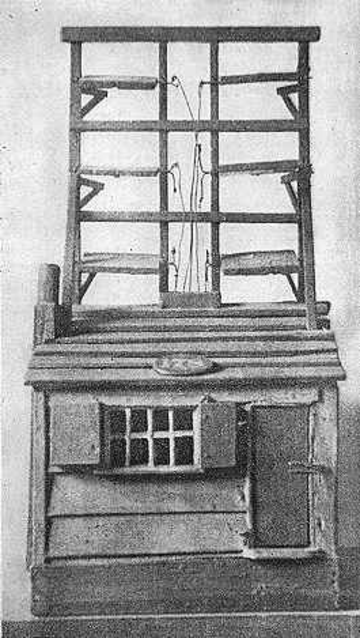
\includegraphics[scale=0.25]{./pics/shuttercabin}\cite{klappentelegraph}
		\hspace{25pt}
	 	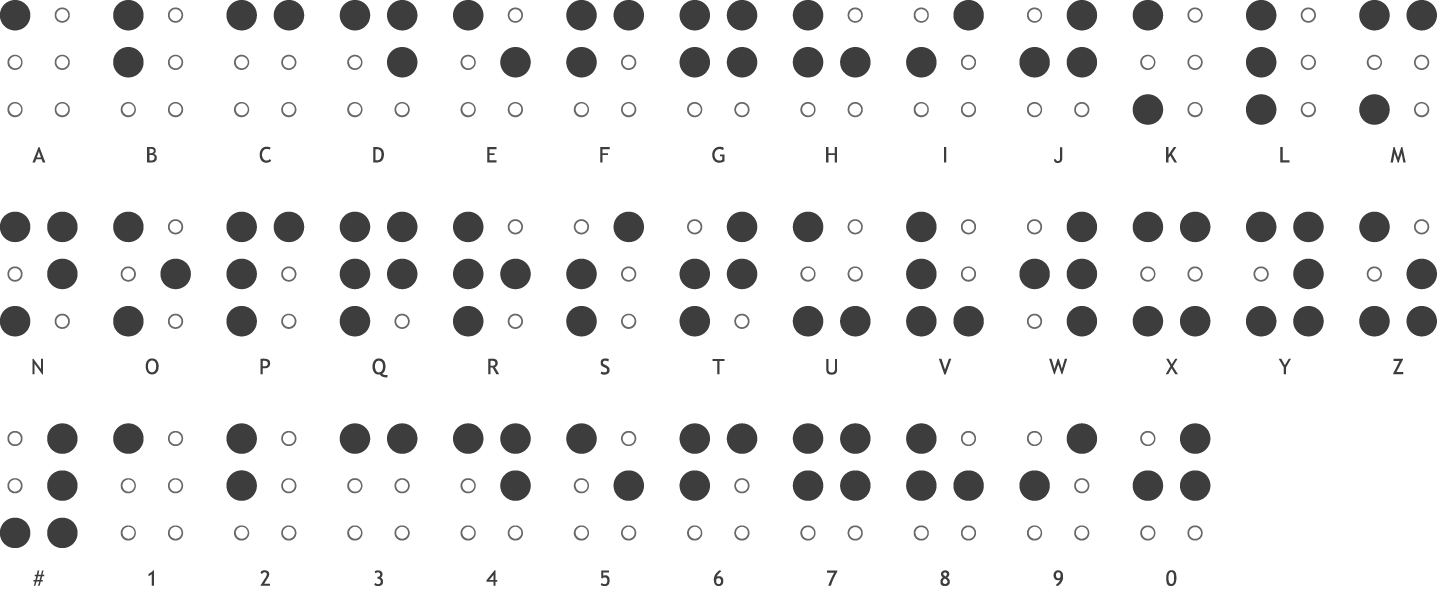
\includegraphics[scale=0.17]{./pics/braille}\cite{braille}
	 	\caption{Links sieht man einen Klappentelegraphen. Rechts das englische Braille-Aphabet. }
	  	\label{fig:braille}
	\end{figure}
\newpage
\section{Theoretische Grundlagen}

Im Folgenden werden Datenstrukturen und Operationen eingeführt, die wir in dieser Arbeit benötigen werden.

\subsection{Operationen auf Strings}

Sei das Alphabet $\Sigma$ definiert als eine Menge von Zeichen, dann bezeichnet $\Sigma^{*}$ die Menge aller Worte, die aus dem Alphabet gebildet werden können. Jedes dieser Worte bezeichnet man als String.
	Sei $s$ ein String mit der Länge $n$.
	
	\begin{definition}[Länge]
		Sei $|s|$ die Länge des String $s$, das heißt die Anzahl von Zeichen in $s$.
	\end{definition}
	
	\begin{definition}[Leerstring]
		Sei $\varepsilon \in \Sigma$* der leere String. Es gilt $|\varepsilon|$ = 0.
	\end{definition}
	
	\begin{definition}[Symbolzugriff]
		Für $x \in \mathbb{N}$ und $x \leq n$ sei $s[x]$ das $x$-te Zeichen aus $s$.
	\end{definition}
	
	\begin{definition}[Teilstring]
		Für $x,y \in \mathbb{N}$ und $1 \leq x < y \leq n$ sei $s[x,y]$ die Zeichenfolge vom $x$-ten bis zum $y$-ten Zeichen aus $s$. $s$[x] und $s$[y] einschließlich.
	\end{definition}
	
	\begin{definition}[Suffix]
		 Für $x \in \mathbb{N}$ und $x \leq n$ sei $s[x..]$ das $x$-te Suffix von $s$. Also gilt $s[x..] = s[x,n]$.
	\end{definition}
	
\subsection{Suffix-Tree}

\begin{definition}[Suffix-Tree]
		Ein Suffix-Tree eines Strings $s$ ist ein Baum mit $n$ Blättern. Alle inneren Knoten erfüllen folgende Bedingungen:
		\begin{itemize}
			\item Jeder Knoten hat mindestens 2 Kinder.
			\item Jede Kante ist mit einem nicht-leeren Teilstring von $s$ markiert.
			\item Die Markierung ausgehender Kanten eines Knotens beginnen nicht mit dem gleichen Zeichen.
			\item Die Konkatenation von allen Zeichen auf dem Pfad von der Wurzel zum Blatt $i$ ist das $i$-te Suffix $s[i..]$ von $s$.
		\end{itemize}
		\begin{beispiel}[Suffix-Tree]
			$s$ = \texttt{ananas\$}
			\begin{figure}[h]
				\centering
				  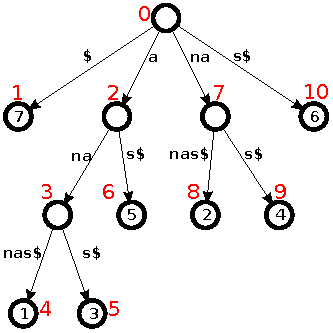
\includegraphics[scale=0.8]{./pics/ananas_suffixTree_inorder}
				  \cite{suffixtreeurl}
				  \caption{Diese Abbildung zeigt den Suffix-Tree zu $s$ = \texttt{ananas\$}. Die Blätter sind hierbei nummeriert. Der String auf dem Pfad von der Wurzel zum Blatt $i$ repräsentiert das Suffix $s[i..]$. Die roten Zahlen an den Knoten sind durch eine Pre-Order-Nummerierung entstanden und sind die IDs der Knoten. }
				  \label{fig:suffixTree}
			\end{figure}
		\end{beispiel}
		
	\end{definition}
	
	
\section{Idee der LZ78 Variante}

Um die Grundidee des Verfahrens, das wir in dieser Arbeit entwickeln, zu erläutern, betrachten wir im Folgenden zunächst LZ78.

\subsection{LZ78}

LZ78 wurde 1978 von Jacob Ziv und Abraham Lempel erfunden und ist ein Verfahren zur Textkompression. Es benutzt dabei ein \textit{adaptives Wörterbuch}. Das heißt es wird je nach Eingabetext ein Wörterbuch erzeugt. Dieses Wörterbuch besteht aus Faktoren, die auf vorherige, längste Vorkommen des selben Substrings verweisen und an diesen ein Zeichen anhängen. Diese Verweise benötigen weniger Speicher als der Originaltext, wodurch es zu einer Kompression kommt.\cite[S.53ff]{managingGigabytes}

Der (naive) Algorithmus durchläuft den String bzw. den Eingabetext $T$ und ersetzt Redundanzen durch Verweise auf das längste vorherige Vorkommen des selben Teils und hängt das nächste Zeichen an diesen Verweis an. Dadurch wird ein Baum erzeugt, der sog. LZ78-Trie. Dieses Verfahren wird nun am Beispiel von $T$ = \texttt{ananas\$} verdeutlicht.\newpage
 	
	\begin{figure}[h]
	\begin{tabular}[t]{cc}
		\begin{tabular}[b]{l c c c c c}\hline
			& 1 & 2 & 3 & 4 & 5 \\ \hline
		   Textteil & \texttt{a} & \texttt{n} & \texttt{an} & \texttt{as} & \texttt{\$}\\ \hline
		   Faktorzerlegung & (-,\texttt{a}) & (-,\texttt{n}) & (1,\texttt{n}) & (1,\texttt{s}) &  (-,\texttt{\$})\\ \hline
		\end{tabular} & 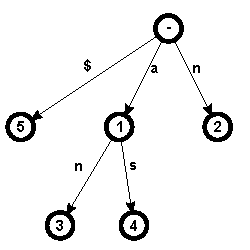
\includegraphics{./pics/ananas_LZ78Tree}
	\end{tabular}
	\caption{Links sieht man die Faktorisierung nach LZ78 und rechts den entsprechenden LZ78-Tree. Der $i$-te Faktor $(x,s)$ wird zu einem neuen Knoten $i$ mit $x$ als Elternknoten und die Kante $(x,i)$ wird mit $s$ beschriftet.}
	\label{fig:lz78}
	\end{figure}

\begin{definition}[Faktor (LZ78)]
	Ein \textit{Faktor} ist ein Tupel $(x,s)$ mit $x \in \{1..z\} \cup \{-\}$ und $s \in \Sigma$. $x$ bezeichnet hierbei den Elternknoten im LZ78-Tree und $s$ die Kantenbeschriftung der Kante von $x$ zum neu entstehenden Knoten. $z$ ist die Anzahl der Faktoren. Die Zahlen in den Knoten stehen für die Faktoren.
\end{definition}	
	

\subsection{LZ78 Variante}	

Im Gegensatz zu LZ78 kann diese Variante (im Folgenden LZ78V genannt) auch mehr Zeichen an eine Ersetzung anhängen.
	Im Beispieltext $T$ = \texttt{ananas\$} folgt nach einem \texttt{'n'} immer ein \texttt{'a'}. Dies spiegelt sich im Suffix-Tree\ref{fig:suffixTree} durch die Kantenbeschriftung \texttt{'na'} wider. Mit LZ78V können wir nun beim ersten Lesen von \texttt{'n'} den Faktor (-,\texttt{na}) erstellen, denn nach \texttt{'n'} kann nichts anderes kommen. Es ergibt sich folgende Faktorzerlegung:\\
	\begin{figure}[h]
	\begin{tabular}[t]{c c c}
		\begin{tabular}[b]{l c c c}\hline
			& 1 & 2 & 3  \\ \hline
  		Textteil & \texttt{a} & \texttt{na} & \texttt{nas\$} \\ \hline
  		Faktorzerlegung & (-,\texttt{a}) & (-,\texttt{na}) & (2,\texttt{s\$}) \\ \hline
		\end{tabular} & \hspace{2cm} & 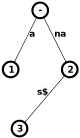
\includegraphics{./pics/ananas_LZ78VTree}\\\\
	\end{tabular}
	\caption{Links sieht man die Faktorisierung nach LZ78V und rechts den entsprechenden LZ78V-Tree. Der $i$-te Faktor $(x,s)$ wird zu einem neuen Knoten $i$ mit $x$ als Elternknoten und die Kante $(x,i)$ wird mit $s$ beschriftet. Im Gegensatz zum LZ78-Tree kann $s$ aber mehr als ein Zeichen beinhalten.}
	\label{fig:lz78v}
	\end{figure}
	
	Den LZ78V-Tree können wir mit einem zweidimensionalen Array $A$ repräsentieren. So wäre $A[i][1] = x$ und $A[i][2] = s$ der $i$-te Faktor $(x,s)$ in der Array-Darstellung. Im Beispiel $T$ = \texttt{ananas\$} ergibt sich:\\\\
	\begin{tabular}{l c c c}
						\hline
							& 1 & 2 & 3 \\\hline
						$A[1]$ & - & - & 2 \\\hline
						$A[2]$	& \texttt{a} & \texttt{na} & \texttt{s\$}\\\hline
						
			
	\end{tabular}
	


 

	
\newpage

\bibliography{bibAngaben}	

\end{document}